\documentclass{../talk}

\title{Diode Laser Absorption Spectroscopy of Rubidium}
\author[Iago B. Mendes]{Iago B. Mendes \\ Lab partner: Avay Subedi}
\date{March 20, 2025}

\begin{document}

\maketitle

\section{Introduction}

\begin{frame}{Motivation}
  \begin{itemize}
    \item Study hyperfine splitting of the ground state of rubidium ($^{85}$Rb and $^{87}$Rb)
    \item<2-> Measure it using absorption spectroscopy
    \item<3-> Use a diode laser and a Fabry-Perot resonator
    \item<4-> Test consistency of measured hyperfine splittings with literature values
\end{itemize}

\end{frame}

\section{Theory}

\begin{frame}{Energy splittings}
  \begin{multicols}{2}
    \begin{itemize}
      \item<2-> $^{85}$Rb and $^{87}$Rb outermost electron \\
        ground state $\to$ 5s ($\ell = 0$) \\
        excited state $\to$ 5p ($\ell = 1$)
      \columnbreak
      \item<3-> Spin-orbit interaction $\to$ fine splitting \\
        different excitations: $D_1$ and $D_2$
      \item<4-> Electron-nucleus interaction $\to$ hyperfine splitting
    \end{itemize}
  \end{multicols}
  \begin{figure}
    \centering
    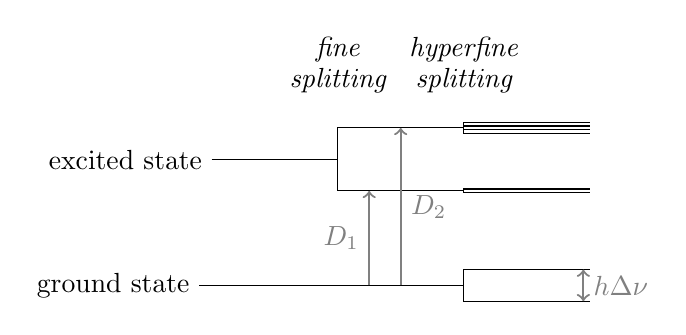
\begin{tikzpicture}[scale=0.8]
      \draw (-0.2,0) node[anchor = east] {ground state} -- (4,0);
      \draw (4,0) -- (4,0.25) -- (6,0.25);
      \draw (4,0) -- (4,-0.25) -- (6,-0.25);
  
      \node at (2,3.75) {\em fine};
      \node at (2,3.25) {\em splitting};
      \node at (4,3.75) {\em hyperfine};
      \node at (4,3.25) {\em splitting};
  
      \draw (0,2) node[anchor = east] {excited state} -- (2,2);
      \draw (2,2) -- (2,2.5) -- (4,2.5);
      \draw (2,2) -- (2,1.5) -- (4,1.5);
      \draw (4,2.5) -- (4,2.59) -- (6,2.59);
      \draw (4,2.5) -- (4,2.53) -- (6,2.53);
      \draw (4,2.5) -- (4,2.47) -- (6,2.47);
      \draw (4,2.5) -- (4,2.41) -- (6,2.41);
      \draw (4,1.5) -- (4,1.53) -- (6,1.53);
      \draw (4,1.5) -- (4,1.47) -- (6,1.47);
  
      \draw[->, thick, color=gray] (2.5,0) -- (2.5,1.5) node[pos = 0.5, anchor = east] {$D_1$};
      \draw[->, thick, color=gray] (3,0) -- (3,2.5) node[pos = 0.5, anchor = west] {$D_2$};
  
      \draw[<->, thick, color=gray] (5.9,-0.25) -- (5.9,0.25) node[pos = 0.5, anchor = west] {$h \Delta \nu$};
    \end{tikzpicture}
    \caption{}
  \end{figure}
\end{frame}

\begin{frame}{Absorption spectroscopy}
  \begin{itemize}
    \item The beam passes through a vapor cell containing rubidium atoms
    \item<2-> If the laser frequency matches an atomic transition ($D_2$):
      \begin{itemize}
        \item Atoms absorb photons, exciting electrons to higher energy states
        \item Absorbed photons are re-emitted in random directions (scattering)
        \item Reduced intensity in the original beam path is measured as absorption
      \end{itemize}
    \item<3-> Transmission spectrum shows dips at resonant frequencies
\end{itemize}

\end{frame}

\section{Methods}

\begin{frame}{Diode laser}
  \begin{itemize}
    \item Semiconductor laser diode used to generate tunable laser beam
    \item<2-> Wavelength tuning: change current \\
      $\Rightarrow$ change frequency
    \item<3-> $\lambda \sim$ 780 nm \\
      $\Rightarrow$ sweep current over time to get all peaks
\end{itemize}

\end{frame}

\begin{frame}{Fabry-Perot resonator}
  \begin{itemize}
    \item Transmits only specific frequencies based on mirror spacing
    \item<2-> Used to measure discrete transmission peaks
    \item<3-> Peak frequency spacing: free spectral range (FSR)
      \begin{equation}
        \Delta \nu_\text{FSR} = \frac{c}{2 n L}
      \end{equation}
    \item<4-> Enables time-to-frequency conversion
  \end{itemize}
\end{frame}

\section{Results}

\begin{frame}{Transmission and absorption data}
  \begin{itemize}
    \item<2-> Manually selected the times for each transmission peak
    \item<3-> Used Igor Pro to fit to a function for the cummulative number of peaks at a given time
      \begin{equation}
        N(t) = K_0 + K_1 t + K_2 t^2 + K_3 t^3
      \end{equation}
  \end{itemize}
  \begin{figure}
    \centering
    \includegraphics[width=0.6\textwidth]{data/time_plot.pdf}
    \caption{}
  \end{figure}
\end{frame}

\begin{frame}{Time-to-frequency conversion}
  \begin{itemize}
    \item<2-> Length of Fabry-Perot resonator
      \begin{equation}
        L = 900(1) \text{ mm}
      \end{equation}
    \item<3-> Free spectral range
      \begin{equation}
        \Delta \nu_\text{FSR} = \frac{c}{2 n L}
      \end{equation}
    \item<4-> Frequency spacing between transmission peaks is uniform
      \begin{equation}
        \nu(N) = \Delta \nu_\text{FSR} N + \nu_0
      \end{equation}
    \item<5-> Conversion function
      \begin{align}
        \nu(t)
        &= \Delta \nu_\text{FSR} N(t) + \nu_0 \\
        &= \Delta \nu_\text{FSR} (K_0 + K_1 t + K_2 t^2 + K_3 t^3) + \nu_0
      \end{align}
  \end{itemize}
\end{frame}

\begin{frame}{Absorption spectrum}
  \begin{multicols}{2}
    \begin{itemize}
      \item<2-> Gaussian fits with {\tt scipy}
      \item<3-> Note: misalignment of peak offsets
      \columnbreak
      \item<4-> Used literature values to identify peaks
        \begin{align*}
          \text{2nd and 3rd} &\to {}^{85}\text{Rb} \\
          \text{1st and 4th} &\to {}^{87}\text{Rb}
        \end{align*}
        \vspace*{-1cm}
    \end{itemize}
  \end{multicols}
  \begin{figure}
    \centering
    \includegraphics[width=0.6\textwidth]{data/analysis.pdf}
    \caption{}
  \end{figure}
\end{frame}

\begin{frame}{Hyperfine splittings}
  \begin{itemize}
    \item Measurements
      \begin{align}
        \Delta\nu(^{87}\text{Rb}) &= 6.5(5) \text{ GHz} \\
        \Delta\nu(^{85}\text{Rb}) &= 2.9(3) \text{ GHz}
      \end{align}
    \item<2-> Literature values\footnote{D. A. Steck, Alkali D Line Data.}
      \begin{align}
        \Delta\nu_\text{literature}(^{87}\text{Rb}) &= 3.035732439(6) \text{ GHz} \\
        \Delta\nu_\text{literature}(^{85}\text{Rb}) &= 6.83468261090429(9)) \text{ GHz}
      \end{align}
  \end{itemize}
\end{frame}

\begin{frame}{Peak widths}
  \begin{itemize}
    \item Expected width due to Doppler broadening for 780 nm laser\footnote{J. R. Brandenberger, Experiments in Laser Physics and
    Spectroscopy for Undergraduates.}
      \begin{equation}
        \delta\nu_\text{Doppler} = 502 \text{ MHz}.
      \end{equation}
    \item<2-> Full-width at half-maximum (FWHM)
      \begin{equation}
        \delta\nu_\text{FHHM} = 2 \sqrt{2 \ln 2} \ \sigma_\text{Gaussian}
      \end{equation}
    \item<3-> Measurements
      \begin{align}
        \delta\nu_1 &= 520(10) \text{ MHz}, \\
        \delta\nu_2 &= 590(6) \text{ MHz}, \\
        \delta\nu_3 &= 570(20) \text{ MHz}, \\
        \delta\nu_4 &= 490(90) \text{ MHz}.
      \end{align}
  \end{itemize}
\end{frame}

\section{Conclusion}

\begin{frame}{Summary}
  \begin{itemize}
    \item Successfully measured hyperfine splitting for $^{85}$Rb and $^{87}$Rb
    \item Results consistent with literature values within experimental uncertainty
    \item Peak width measurements affected by Doppler broadening and misalignment
    \item Possible improvements:
      \begin{itemize}
        \item Adjust diode laser parameters to align peak offsets
        \item Improve frequency resolution with better laser stability
      \end{itemize}
\end{itemize}

\end{frame}

\begin{frame}{The end}
  \textbf{\Large Thank you! Any questions?}
  
  \hrulefill
\end{frame}

\end{document}
